\documentclass[notumble,combine]{leaflet}
\usepackage[dvipsnames,usenames]{color}
\usepackage{graphicx}
\usepackage{alltt}
\usepackage{url}
\usepackage{ascmac}
\usepackage{comment}
\usepackage{here}
\usepackage{wrapfig}
\usepackage{floatflt}

\makeatletter
% Section color
%% from leaflet.cls
\renewcommand\section{\@startsection{section}{1}{\z@}%
  {-3.5ex \@plus -.75ex}%
  {1ex} %{1.5ex}%
  {\normalfont\large\sectfont\color{NavyBlue}}}
\renewcommand\subsection{\@startsection{subsection}{2}{\z@}%
  {-2.5ex plus -.5ex}%
  {1\p@} %{1ex}%
  {\normalfont\normalsize\sectfont\color{Green}}}
\makeatother

\graphicspath{{figures/}} 

\title{
	\includegraphics[width=\textwidth]{facebook_banner}\\
        \parbox[c]{2cm}{\resizebox{2cm}{!}{\textcolor{red}{\bf{@}}}}\\
	\includegraphics[width=\textwidth]{osc2016-kyoto-logo}\\
	\vfill
	\parbox[c]{\textwidth}{\includegraphics[width=\textwidth]{daimonji}}\\
        \vfill
	\resizebox{7cm}{!}{\bf 関西*BSDユーザ会}\\
        \resizebox{6cm}{!}{{\bf \url{http://www.kbug.gr.jp/}}}\\
        
\includegraphics[width=2cm]{kbug.gr.jp.eps}\\
        \resizebox{7cm}{!}{2016年7月29日(金),30日(土)}\\
}

\date{}

\begin{document}
\maketitle

\thispagestyle{empty}
\pagebreak{}
\section{関西*BSDユーザ会(K*BUG)ってなぁに?}
関西 *BSD ユーザ会 (Kansai *BSD Users Group; K*BUG)とは、
BSD系OSのユーザ同士の情報交換のための{\Large\em \textcolor{red}{場}}で、1999年に設立されました。

年に数度の勉強会やイベントへの参加、そして{\Large\em \textcolor{red}{飲み会}}を行っています。

\subsection{K*BSDの基本理念}
K*BUGの基本理念はのとおりです。

\fbox{\begin{minipage}{\textwidth}
\begin{itemize}
\item 場の提供を目的とする
\item 人のケツは叩くが足は引っ張らない
\item 来るものは拒まず、猿ものは追わず
\item だれでも役員になれる。誰でも役員は止められる
\end{itemize}
\end{minipage}}

少し難しく感じるかもしれないですが、
\textcolor{red}{\bf\Large BSDへの愛と情熱}
があれば、
あなたが
\textcolor{blue}{やりたいと思うことができる場}
がK*BUGなのです。

\section{K*BUG Keywords}
K*BUGでは、以下のようなKeywordに関する発表や展示が行われています。

{\large\bf\textcolor{red}{{BSD}}} (FreeBSD (PC-BSD), NetBSD, OpenBSD, DragonlyBSD, {\footnotesize Mac OS X(?), iOS(??) }, ...)
の更新情報 / 利用方法 / ...,
arch (i386, amd64, arm (Raspberry Pi), macppc, landisk, zaurus, wzero3, hpcmips, netwalker, ipaq, fonera, vax, ...),
kernel hackや新技術 (DTrace, ZFS, シリアルドライバ, ...),
FreeBSD portsってなに? (portsの作り方, redports, ...),
Security (実際のセキュリティ問題に関して, セキュリティを向上するために, ...), 
教育,
いろいろな言語 (Prolog, Lisp, awk, Squeak, Scratch, ...),
OpenCV,
ContaoCMS, 
hardware (UPS, HDD, Server, Bluetooth, GPIO, ...),
ものづくり,
電子工作,
ニコ動技術部 (猫耳サーボ (USB audio servo controler)
, ...),
雑誌付録基板 ,
Physical Computing (Gainer (gainerm-lib), Arduino, ...),
木彫, でーもんくん, でもんむし君 , \\
\hfill{\textcolor{red}{{\bf\large 飲み会}}}, and {\em\textcolor{red}{{ more with }}{\Large\bf\textcolor{red}{{YOU!!}}}}

\newpage
\section{K*BUGの活動}
最近の活動はこんな感じです。
もし、興味のあるテーマがあったら、
\begin{center}
{\huge\bf \textcolor{red}{遊びに来てね!!}}
\end{center}

\subsection{2016年6月18日(土)@京都 第3回研究会}
\begin{itemize}
\item NetBSDをsysupgradeで更新
\item Bluetooth LE Mouse on FreeBSD
\item おっさん porter のリハビリ
\item pkgsrc on OS X 10.11
\end{itemize}

\subsection{2016年4月23日(土)@大阪 第2回研究会}
\begin{itemize}
\item XIJな話
\end{itemize}

\subsection{2016年2月20日(土)@京都 第1回研究会}
\begin{itemize}
\item マシンが増えた場合の管理方法について
\item 今さらsh(1)で作ってみた
\item 宅内ネットワークトラブル
\item efiの話
\item DNSの名前怪傑エラー(現在進行中)
\end{itemize}

\subsection{2016年1月23日(土)@大阪\\\hfill 第17回定期総会 + 併設研究会}
\begin{itemize}
\item sshdのログの傾向
\item こんなん買いました: FIOD U2F
\item iPad \& Apple Configuratorよもやま話
\item 2015年版AAJ
\end{itemize}

\subsection{2015年10月24日(土)@京都 第5回研究会}
\begin{itemize}
\item 京都醸造所試飲スペースの報告
\item FreeBSDをVirtualBoxにインストールしてみた
\item Apple Configurator 2についての軽いデモなど
\end{itemize}

\subsection{2015年8月22日(土)@大阪 第4回研究会}
\begin{itemize}
%\item 会場の説明
\item CIM技術研究会の取り組み
\item (番外) Wi-Fiにつながらない問題、異なるIPアドレスが割り当て
\item 大学のサーバーの更新
\item 「エノキサンタスケテ」の呪文を唱えたこと
\item 今さらZFS (デモあり)
\item Letsencrypt.orgについて
\end{itemize}

\subsection{2015年8月7日(金), 8日(土)@京都\\\hfill OSC2015 Kansai@Kyoto}
\begin{itemize}
\item NetBSD distccを使ったpkgsrcの分散コンパイル環境
\item FreeBSD 11-currentでMZTX-PI-EXT表示
\end{itemize}

\subsection{2015年6月27日(土)@京都 第3回研究会}
\begin{itemize}
\item Bluetooth LE
\item ゆるいpkgsrcの
\item LT的話
  \begin{itemize}
  \item linuxのBluetooth LEで相談
  \item raidframeと壊れたディスク、bootは不可問題
  \item Gdev: Open Source のGPGPU Runtime and Driver Software
  \item Dellの4KディスプレイがFreeBSDで使えへん問題
  \end{itemize}
\item 謎言語
\end{itemize}

\subsection{2015年5月16日(土)@京都 第2回研究会}
\begin{itemize}
\item 今さら sh
\end{itemize}

\subsection{2015年3月7日(土)@大阪 第1回研究会}
\begin{itemize}
%\item うめきた9Fオフィスの紹介
\item blink1について
\item FreeBSDでRaspberry  PIでGPIO
\item 周回遅れの HTTP/2
\item iPadに関する軽い話
\end{itemize}

\section{これからの関連イベント(予定)}
K*BUGでは、2ヶ月に1度程度の頻度で勉強会を行っています。
また、主に関西のイベントで、展示などを行っています。

現在、予定されているイベントは、以下のとおりです。
詳細は、K*BUGのWebページをご確認ください。

\begin{itemize} 
\item 2016年8月20日(土)@大阪 第4回研究会
\item 2016年10月22日(土)@大阪 第5回研究会
\item 2016年11月11日(金),12日(土) KOF2016: 未定
\item 2016年12月10日(土)@京都\\
  \hfill 第18回定期総会 + 併設研究会
\end{itemize}

\section{写真集}
\subsection{OSC2015 Kansai@Kyoto}
    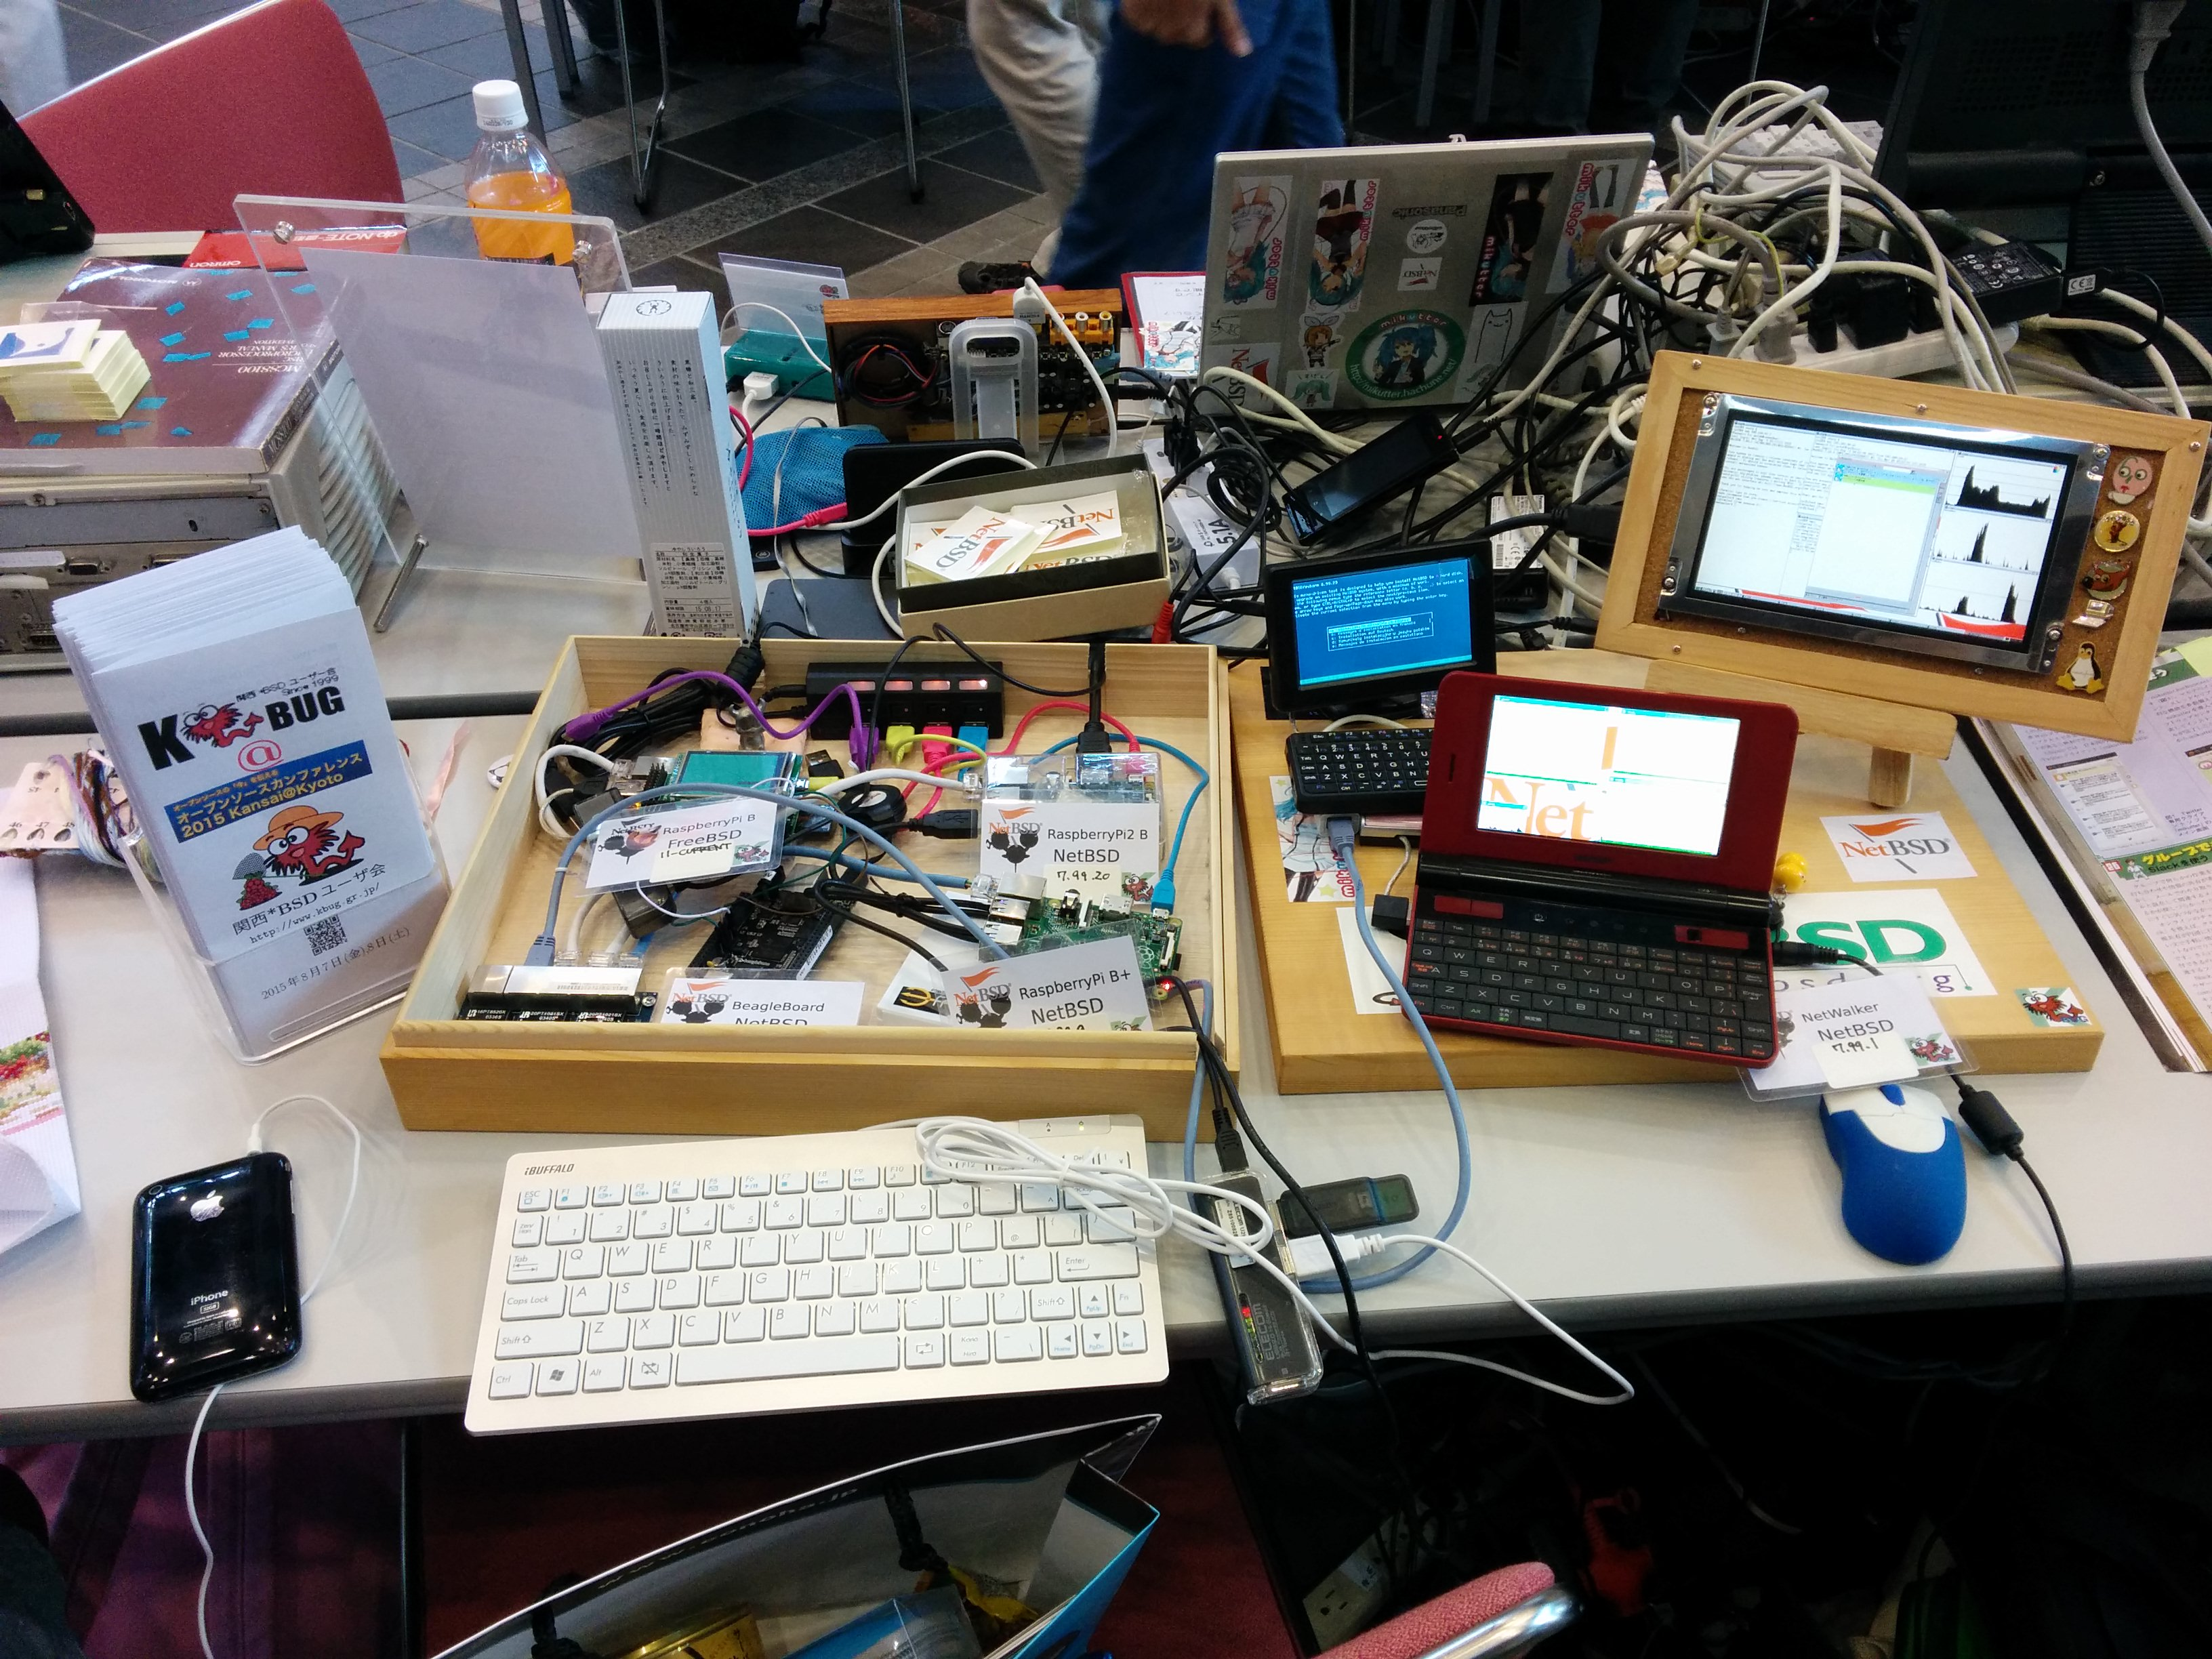
\includegraphics[width=3.5cm]{osc2015-kyoto-booth}
    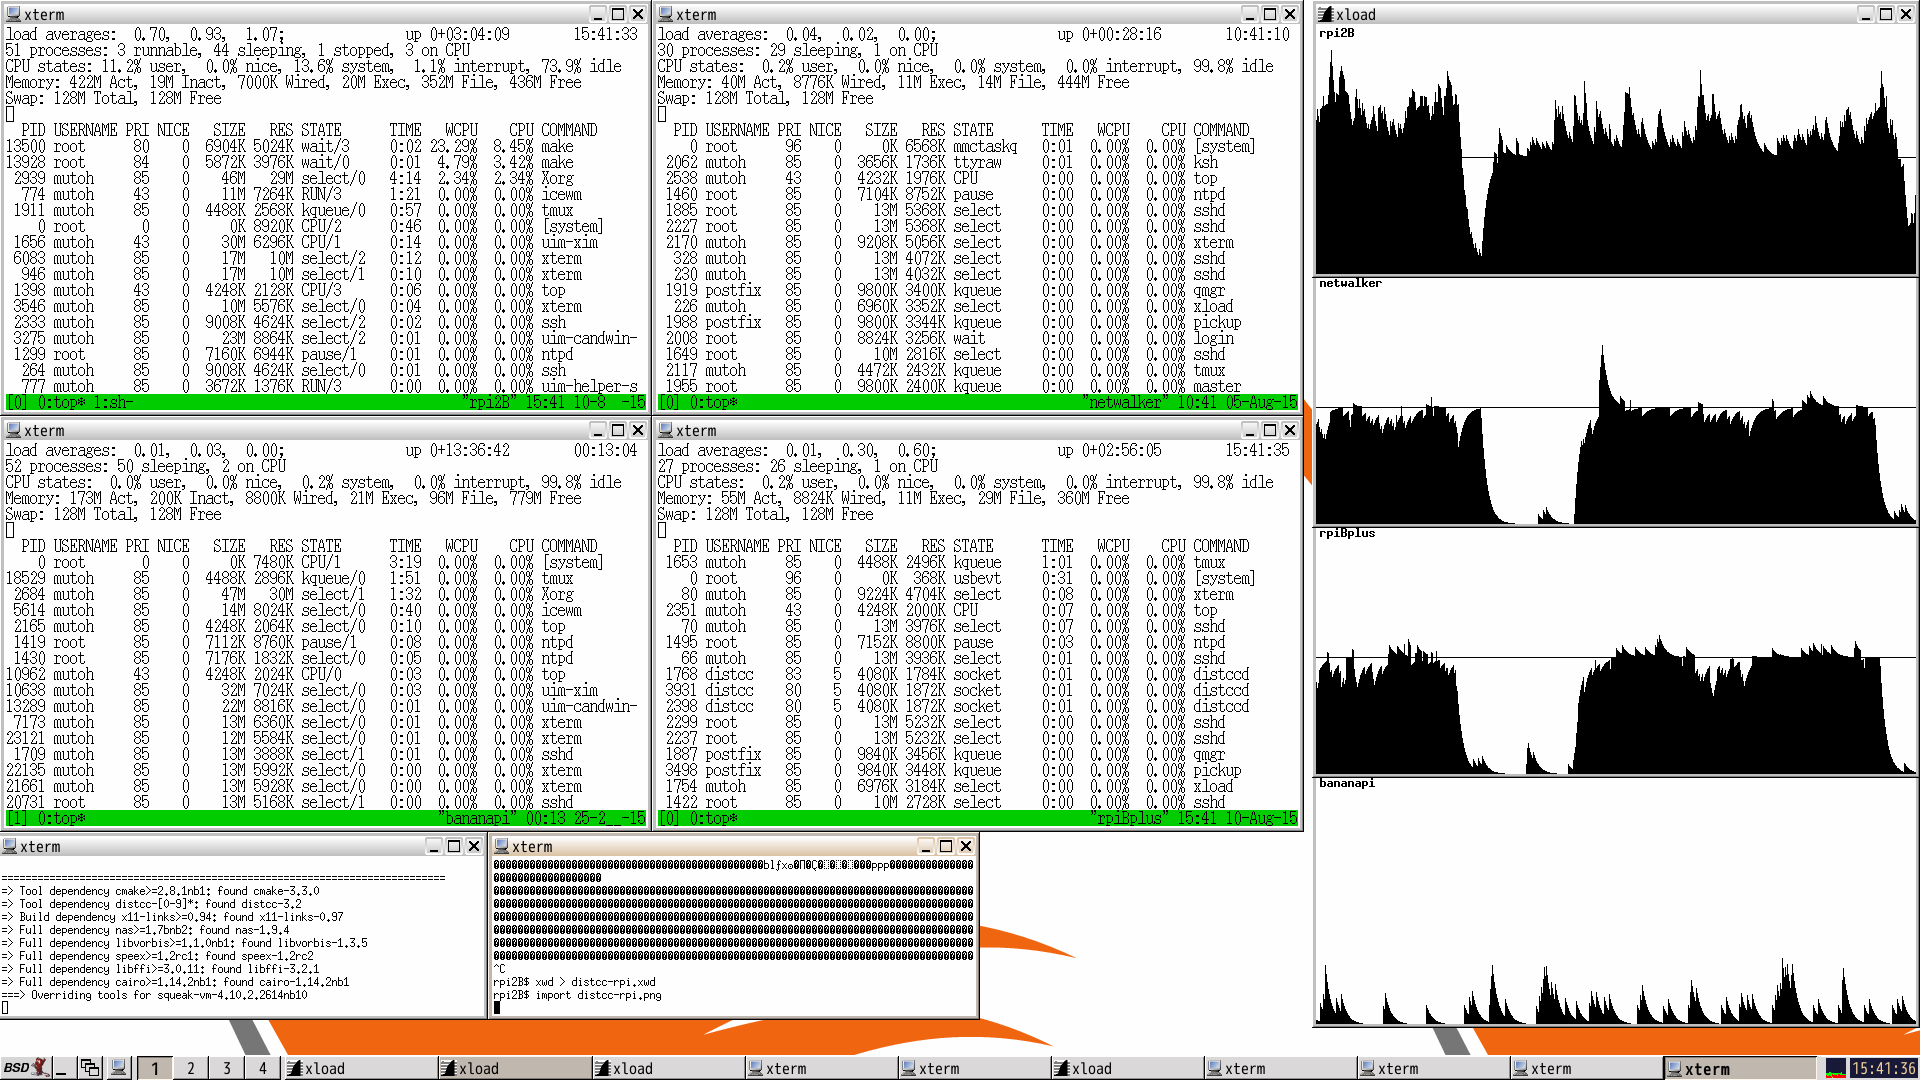
\includegraphics[width=4.5cm]{distcc-rpi}

\subsection{OSC2013 Kansai@Kyoto}
    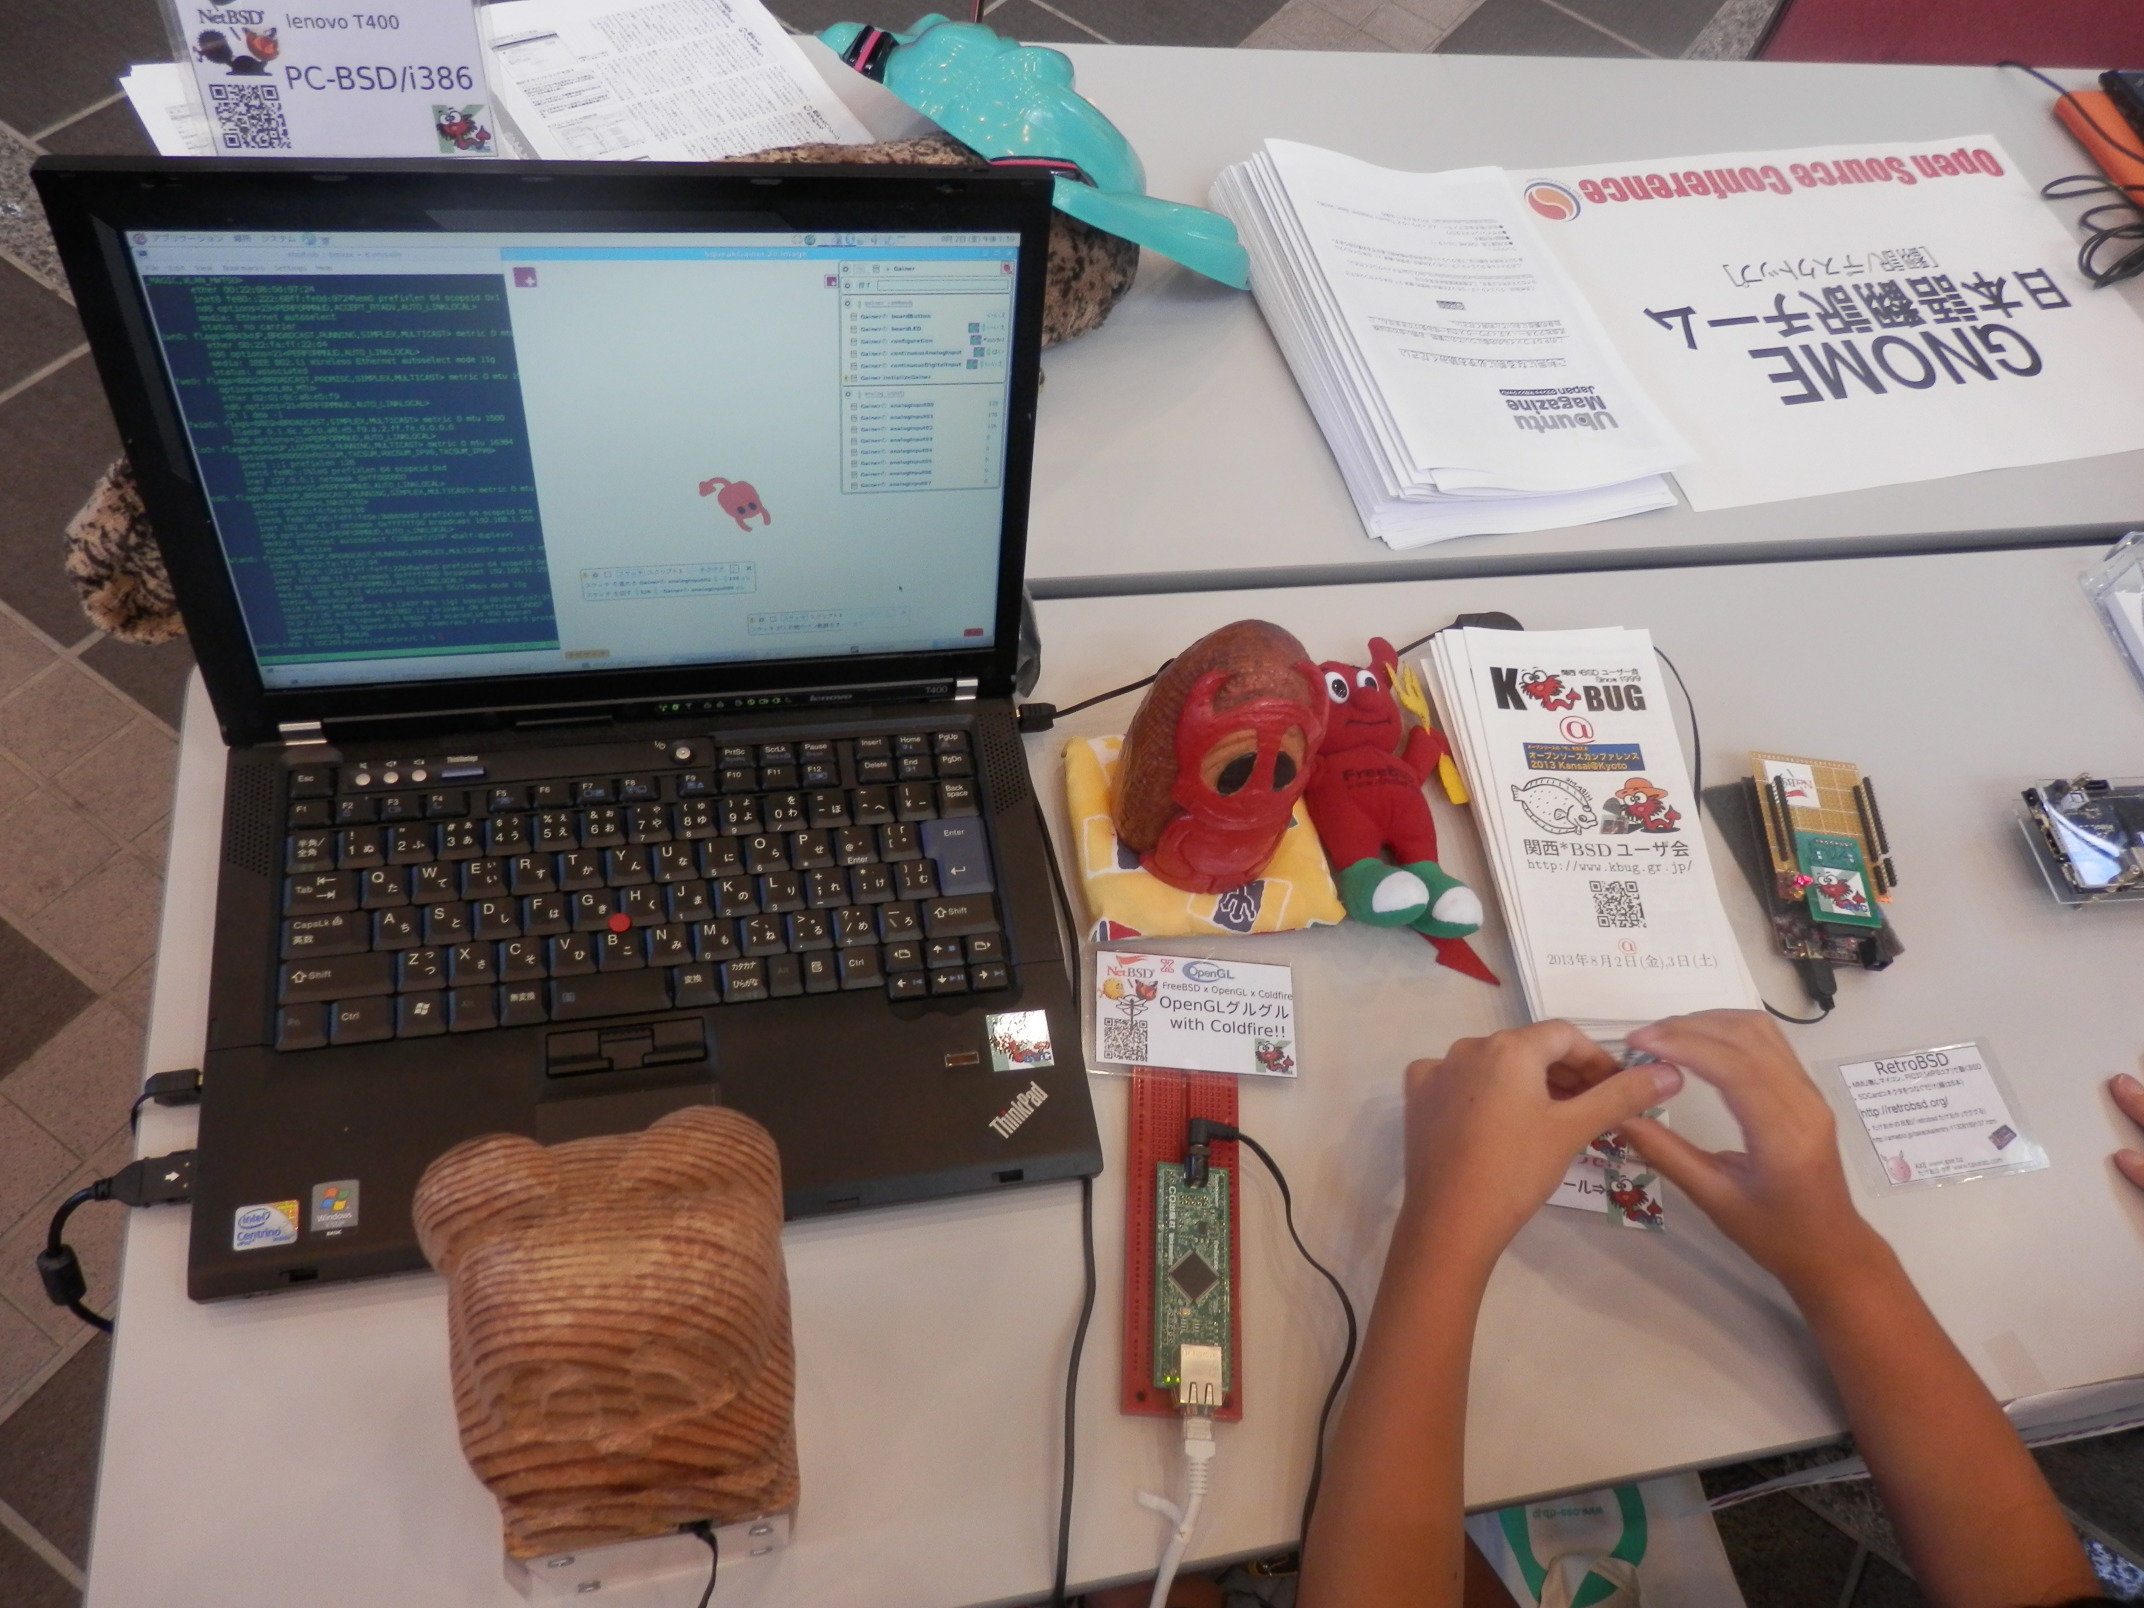
\includegraphics[width=4cm]{osc2013kyoto}
    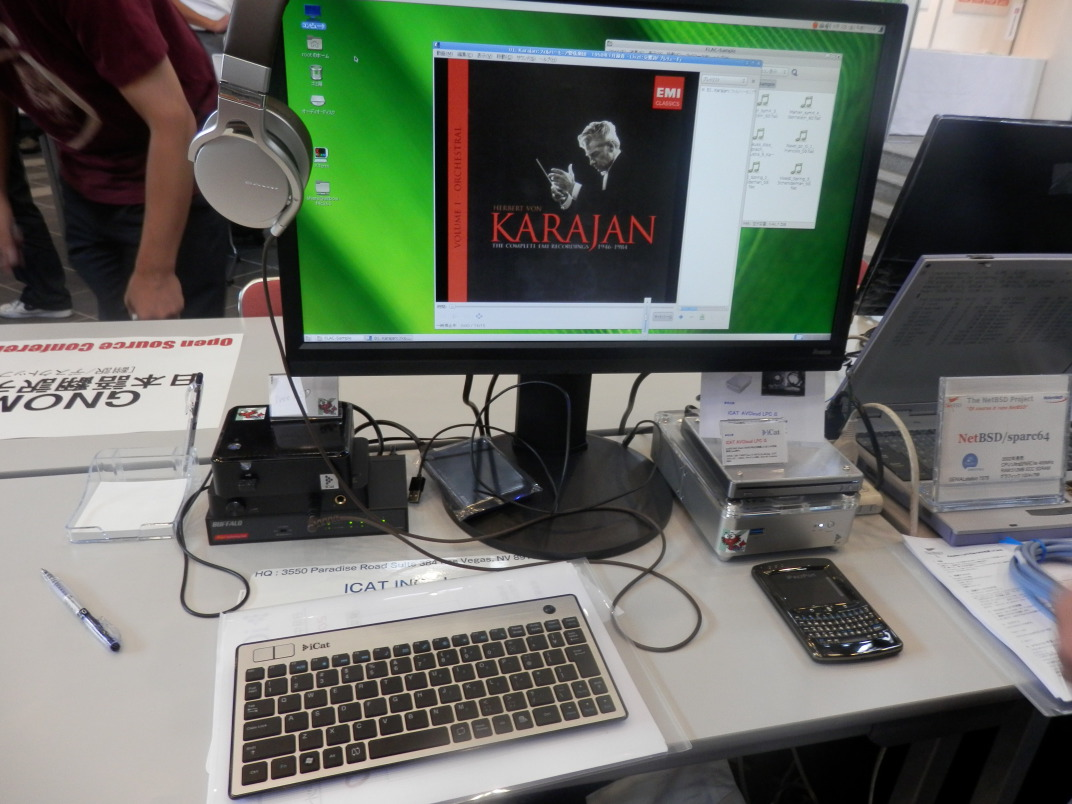
\includegraphics[width=4cm]{osc2013icat}

    \begin{center}
      \includegraphics[width=6cm]{MyKyotoIchiba}
    \end{center}

\newpage
\section{K*BUG @ OSC2016 Kyoto}
K*BUGは、今回以下のような活動で参加しています。

\subsection{ブース展示}
「K*BUG + 中村和志(個人)」として、以下の様なブース展示を行っています。
\begin{itemize}
\item RetroBSDとLiteBSD
\item Raspberry Piと仲間たちのdistccコンパイルクラスタ
\end{itemize}

\subsection{チラシとシールの配布} % by 日本NetBSDユーザーグループ}
このチラシとK*BUGシール
を配布しています。

\subsection{JNUGセミナー: NetBSDのご紹介}
NetBSDは、自由に利用可能で、BSDライセンスに基づき再配布可能なUNIX-likeオペレーティングシステムです。
NetBSDの概要および最近の動向をご紹介します。

\begin{itemize}
\item 日時: 2016年7月29日(金) 16:15-17:00
\item 会場: 1号館4F A会議室
\item 講師:蛯原 純(The NetBSD Project,developer )ら
\item 対象者:コンピュータとかゲーム機とかシャープとかオムロンとか好きな人。
\end{itemize}

%\begin{center}
% 
\includegraphics[width=4cm]{oval-seal-4}
%\end{center}

\vfill
\begin{minipage}{\textwidth}
\begin{boxnote}

\section{kbug-usersメーリングリスト}
K*BUGでは、K*BUGメンバーの情報交換や、イベントなどの情報伝達用に
kbug-usersメーリングリストを用意しています。

K*BUGメンバーは、基本的にはこのメーリングリストを読んでいることが期待
されます。

購読は、% 右のQRコードを使うか、
このURL
\footnote{\scriptsize \url{http://www.kbug.gr.jp/kbug-mailing-lists.html}}
をご参照ください。
\end{boxnote}
\end{minipage}
\vfill
\hfill
{\footnotesize\input{date.tex}}
\end{document}
